\begin{figure}[tb]
\centering
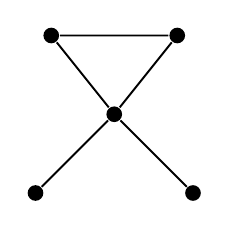
\begin{tikzpicture}[
  vertex/.style={circle,fill,inner sep=2pt},
  line width=.7pt,
]
\node[vertex] (centre) at (0,0) {};
\node[vertex] (upperleft) at (-.8,1) {};
\node[vertex] (upperright) at (.8,1) {};
\node[vertex] (lowerleft) at (-1,-1) {};
\node[vertex] (lowerright) at (1,-1) {};
\draw (centre)--(upperleft)--(upperright)--(centre);
\draw (lowerleft)--(centre)--(lowerright);
\end{tikzpicture}
\caption{The cricket graph $B$.}
\label{fig:cricket}
\end{figure}
